\section{Lecture 10: Step Potential}

\begin{align*}
    \qty[-\frac{\hbar^2}{2m} \derivative{^2}{x^2} + V(x)] \Psi(x) = E \Psi(x)
\end{align*}

Take the following potential:

\[ V(x) = \begin{cases}
   0 & x < 0 \\
   V_0 & x > 0
\end{cases} \]

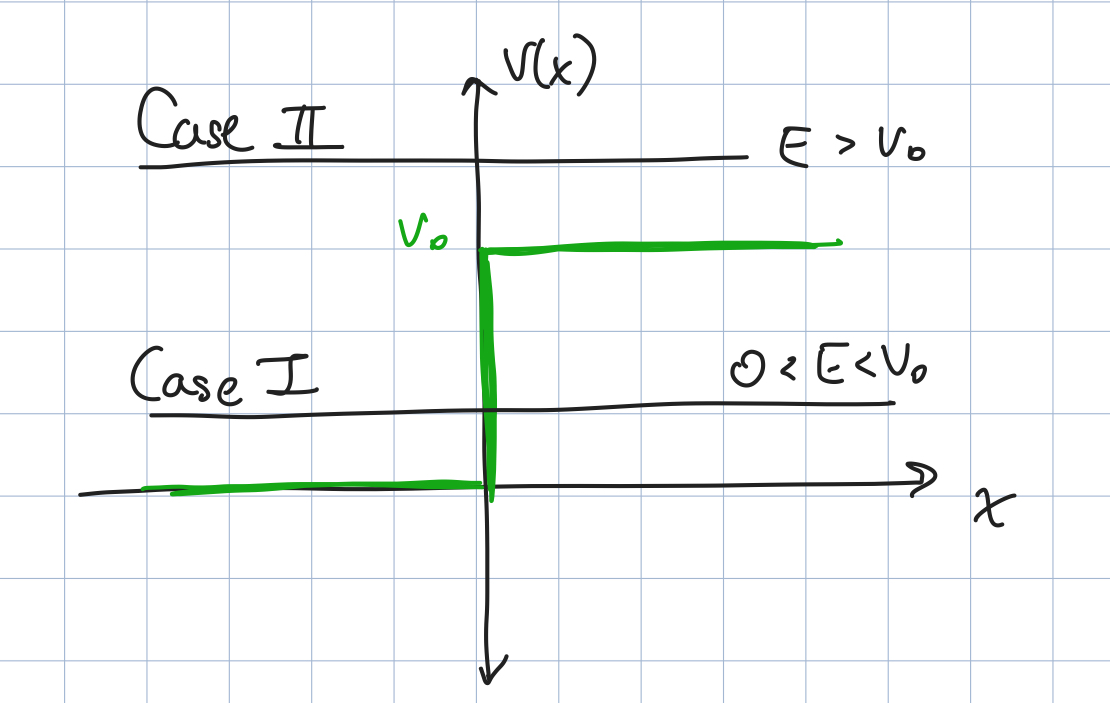
\includegraphics[width=400px]{well.jpeg}

There is no possible solution where $E<0$. In general, the solution is oscillatory in regions where ``it should exist" and dies
out as an exponential in places where ``it shouldn't exist".

Suppose we are in Case I.
For $x < 0$, the equation is, for $k = \qty(2mE/\hbar^2)^{1/2}$
\[ \derivative{^2 \Psi(x)}{x^2} + k^2 \Psi(x) = 0\]
For $x > 0$, the equation is, for $\kappa = \qty(2m(V_0 - E)/\hbar^2)^{1/2}$.
\[ \derivative{^2 \Psi(x)}{x^2} - {\kappa}^2 \Psi(x) = 0\]
The equations have solutions, as we have seen previously, has solution:
\[ \Psi(x) = \begin{cases} Ae^{ikx} + Be^{-ikx} & x < 0 \\ Ce^{\kappa x} + De^{-\kappa x} & x > 0 \end{cases} \]
Now consider the problem of a particle incident from the left. This creates boundary conditions to find the coefficients:

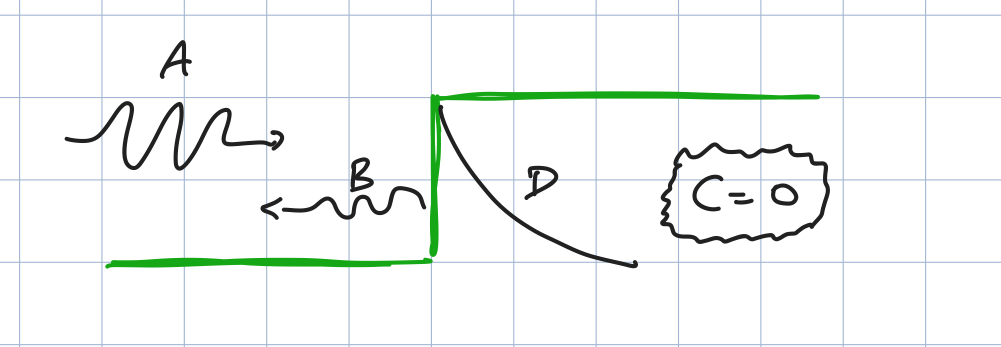
\includegraphics[width=400px]{reflecto.jpeg}

At the sharp interface, we can approximate the wave packet as a plane wave, which is exactly what our solutions do! We need to enforce
continuity of $\Psi, \Psi'$ at $x = 0$. So for $\Psi(0)$ we get the equation $A + B = D$. For $\Psi'(0)$ we get $ik(A - B) = -\kappa D$.
Note that this doesn't uniquely determine the equation since we don't know how high the input amplitude is! So $\frac{B}{A}$ might be a better
variable to define (it is the amplitude fraction). Solving our system yields:
\[ A = \qty(\frac{1 + i\kappa/k}{2})D, B =  \qty(\frac{1 - i\kappa/k}{2})D \]
So:
\[ \frac{B}{A} = \frac{1 - i\kappa/k}{1 + i\kappa/k} = e^{i \alpha} \]
where $\alpha = 2\atan\qty(- \sqrt{\frac{V_0}{E} - 1})$
This has modulus 1! This makes sense because we said none of the wave makes it through and it is all reflected.
Furthermore, $\frac{D}{A} = 1 + e^{i\alpha}$. This means:
\[ \Psi(x) = \begin{cases}
    2Ae^{i\alpha/2} \cos(kx - \frac{\alpha}{2}), x < 0 \\
    2Ae^{i\alpha/2} \cos(\frac{\alpha}{2})  e^{-\kappa x}, x > 0
\end{cases} \]
We define the reflection coefficient as the ratio of the probability currents:
\[ \mathfrak{R} = \frac{|B|^2}{|A|^2} = 1 \]
There is a little bit of probability on the right side, but we don't consider evanescent solutions as actually transmitting the wave. So there is 0 transmittivity.
\[ P(x) = \begin{cases} 
    4 |A|^2 \cos^2 (kx - \frac{\alpha}{2}) & x<0 \\
    |D|^2 e^{-2\kappa x} & x > 0
\end{cases} \]
The probability density to the left of the barrier is oscillatory, despite it being a plane wave. This is because there is self-interference between the wave and its reflected version!

\subsection{Uncertain in the Barrier}
Now we ask, can we observe the particle in the region $x > 0$? For this potential, the decay length is $\frac{1}{\kappa}$.
This observation means we've made a measurement of $\Delta x \sim \frac{1}{\kappa}$. By Heisenberg, this induces an uncertainty in the momentum!
\[ \Delta P_x \geq \frac{\hbar}{\Delta x} \sim \qty[2m(V_0 - E)]^{1/2} \]
But, then $\Delta E = \frac{\qty(\Delta p_x)^2}{2m} \geq V_0 - E$. Which means that we CANNOT SAY the energy is above the barrier.

What happens if the barrier step approaches infinity? The evanescent part disappears. As $V_0 \to \infty$, then $\Psi \to 0$ at the boundary.

Let's step back and take Case II, where $E > V_0$. Similarly,
\[ \Psi(x) = \begin{cases}
    Ae^{ikx} + Be^{-ikx} & x < 0 \\
    Ce^{ik'x} + De^{-ik'x} & x > 0
\end{cases} \]
where $k = \qty(2mE/\hbar^2)^{1/2}$ and $k' = \qty(2m(E - V_0)/\hbar^2)^{1/2}$. Let's again take the case of a left incident wave. $D = 0$ because there is no
back transmission (no other potential barriers), but $A, B, C \neq 0$ since there is the original piece, a reflected piece, and a transmitted piece.
Solving the boundary conditions gets you:
\[ \frac{B}{A} = \frac{k - k'}{k + k'}, \frac{C}{A} = \frac{2k}{k + k'} \]
and we have:
\[ \mathfrak{R} = \frac{\qty[1 - (1 - \frac{V_0}{E})^{1/2}]^2}{\qty[1 - (1 + \frac{V_0}{E})^{1/2}]^2} \]
So the transmittivity is:
\[ \tau = \frac{v' |C|^2}{v |A|^2} = \frac{4kk'}{(k + k')^2} \]
Note QM always has partial reflection.